% ============================================================
% CHƯƠNG 3: PHƯƠNG PHÁP ĐỀ XUẤT
% ============================================================
\chapter{Phương pháp đề xuất}
\label{chap:methodology}

\section{Tổng quan hệ thống}
\label{sec:system_overview}

Hệ thống nhận dạng cảm xúc giọng nói được xây dựng gồm ba giai đoạn xử lý cốt lõi liên kết chặt chẽ với nhau: (1) Trích xuất đặc trưng từ tín hiệu âm thanh thô thành ma trận Log-Spectrogram, (2) Tiền xử lý dữ liệu và chuẩn hóa dạng ảnh đầu vào, và (3) Huấn luyện và phân loại cảm xúc bằng các kiến trúc CNN tiên tiến. Sơ đồ tổng quan mô tả chi tiết luồng xử lý và mối liên hệ giữa các giai đoạn được thể hiện trong Hình~\ref{fig:system_pipeline}.

\begin{figure}[H]
    \centering
    \resizebox{\textwidth}{!}{%
    \begin{tikzpicture}[
        node distance=0.6cm and 0.4cm,
        block/.style={
            draw,
            rectangle,
            rounded corners=4pt,
            align=center,
            fill=white,
            draw=blue!60!black,
            font=\small,
            minimum height=1.1cm,
            minimum width=2.4cm,
            thick
        },
        input/.style={
            draw,
            rectangle,
            rounded corners=6pt,
            align=center,
            fill=green!5,
            draw=green!50!black,
            font=\small\bfseries,
            minimum height=1.1cm,
            minimum width=2.2cm,
            thick
        },
        data/.style={
            draw,
            rectangle,
            align=center,
            fill=yellow!5,
            draw=yellow!50!black,
            font=\small,
            minimum height=1.1cm,
            minimum width=2.2cm,
            thick
        },
        output/.style={
            draw,
            rectangle,
            rounded corners=6pt,
            align=center,
            fill=red!5,
            draw=red!50!black,
            font=\small\bfseries,
            minimum height=1.1cm,
            minimum width=2.2cm,
            thick
        },
        arrow/.style={
            ->,
            >=stealth,
            thick,
            draw=black!70
        },
        stagebox/.style={
            draw=gray!30,
            fill=gray!5,
            rounded corners=8pt,
            inner sep=10pt,
            thick
        }
    ]
        % Giai đoạn 1: Trích xuất đặc trưng
        \node (audio) [input] {Tín hiệu .wav\\(16 kHz)};
        \node (preemp) [block, right=of audio] {Bộ lọc tiền nhấn\\(Pre-emphasis)};
        \node (stft) [block, right=of preemp] {Biến đổi STFT\\(Cửa sổ Hamming)};
        \node (log) [block, right=of stft] {Log-scale (dB)\\200 băng tần};
        \node (spec) [data, right=of log] {Log-Spectrogram\\($200 \times T$)};
        
        \begin{scope}[on background layer]
            \node (stage1) [stagebox, fit=(audio) (spec), label={[font=\small\bfseries\color{blue!80!black}]above:GIAI ĐOẠN 1: TRÍCH XUẤT ĐẶC TRƯNG (FEATURE EXTRACTION)}] {};
        \end{scope}

        % Giai đoạn 2: Tiền xử lý dữ liệu
        \node (seg) [block, below=of audio, yshift=-1.8cm] {Phân đoạn \& Đệm\\($200 \times 300$)};
        \node (norm) [block, right=of seg] {MinMax \& 3-ch\\(Pseudo-RGB)};
        \node (resize) [block, right=of norm] {Resize \& Z-Score\\($3 \times 256 \times 256$)};
        
        \begin{scope}[on background layer]
            \node (stage2) [stagebox, fit=(seg) (resize), label={[font=\small\bfseries\color{blue!80!black}]above:GIAI ĐOẠN 2: TIỀN XỬ LÝ (PREPROCESSING)}] {};
        \end{scope}

        % Giai đoạn 3: Huấn luyện & Phân loại
        \node (cnn) [block, right=of resize, xshift=1.2cm] {Huấn luyện CNN\\(Transfer Learning)};
        \node (output) [output, right=of cnn] {Phân loại\\4 cảm xúc};
        
        \begin{scope}[on background layer]
            \node (stage3) [stagebox, fit=(cnn) (output), label={[font=\small\bfseries\color{blue!80!black}]above:GIAI ĐOẠN 3: PHÂN LOẠI (CLASSIFICATION)}] {};
        \end{scope}

        % Connections
        \draw [arrow] (audio) -- (preemp);
        \draw [arrow] (preemp) -- (stft);
        \draw [arrow] (stft) -- (log);
        \draw [arrow] (log) -- (spec);
        \draw [arrow] (spec.south) -- ++(0,-0.8) -| (seg.north);
        \draw [arrow] (seg) -- (norm);
        \draw [arrow] (norm) -- (resize);
        \draw [arrow] (resize.east) -- (cnn.west);
        \draw [arrow] (cnn) -- (output);
    \end{tikzpicture}%
    }
    \caption{Sơ đồ tổng quan phân chia luồng xử lý dữ liệu và huấn luyện hệ thống theo các giai đoạn cụ thể}
    \label{fig:system_pipeline}
\end{figure}

Luồng xử lý dữ liệu đầy đủ của hệ thống được mô tả theo sơ đồ toán học như sau:
\begin{equation*}
\text{.wav (16kHz)} \xrightarrow{\text{Pre-emphasis}} x_{\text{flt}}(t) \xrightarrow{\text{STFT}} A(f, t) \xrightarrow{\text{Log (dB)}} S_{\text{dB}}(200 \times T)
\end{equation*}
\begin{equation*}
\xrightarrow{\text{Segment + Pad}} (200 \times 300) \xrightarrow{\text{Normalize + 3ch}} (3 \times 200 \times 300) \xrightarrow{\text{Resize + Z-Score}} (3 \times 256 \times 256)
\end{equation*}


\section{Bộ dữ liệu IEMOCAP}
\label{sec:iemocap_dataset}

\subsection{Giới thiệu}

Bộ dữ liệu \textbf{IEMOCAP (Interactive Emotional Dyadic Motion Capture)} được xây dựng và thu thập bởi phòng thí nghiệm SAIL (Speech Analysis and Interpretation Laboratory) thuộc Đại học Nam California (USC), công bố chính thức vào năm 2008 \cite{busso2008}. Đây là một trong những cơ sở dữ liệu đa phương thức quy chuẩn và được trích dẫn rộng rãi nhất trên thế giới dùng để nghiên cứu nhận dạng cảm xúc tự động. Về thiết lập ghi hình, bộ dữ liệu sử dụng hệ thống bắt chuyển động cơ thể hiện đại (motion capture) để thu thập các biểu cảm vật lý thông qua các điểm đánh dấu (markers) trên khuôn mặt, đầu và tay của diễn viên, đồng thời thu lại tín hiệu âm thanh chất lượng cao (tần số lấy mẫu 16 kHz, định dạng 16-bit mono) thông qua microphone đeo tai riêng biệt cho từng người. Quy mô dữ liệu đạt khoảng 12 giờ dữ liệu thô, được thực hiện bởi 10 diễn viên chuyên nghiệp thuộc đoàn kịch Đại học (gồm 5 nam và 5 nữ) chia làm 5 cặp đối thoại song song tương ứng với 5 phiên hội thoại (Session 1 đến Session 5).

Để kích hoạt các phản ứng cảm xúc tự nhiên nhất, các diễn viên thực hiện các buổi diễn đôi (dyadic interactions) dựa trên hai kịch bản thiết kế sẵn. Thứ nhất là kịch bản hội thoại ngẫu hứng (improvised sessions), nơi các diễn viên được cung cấp một tình huống giả lập cụ thể (ví dụ: tranh cãi về một hóa đơn thanh toán sai, nhận được tin vui trúng tuyển công việc mơ ước, mất đồ đạc cá nhân quan trọng, hoặc đối diện với tin buồn từ gia đình) và tự do đối thoại ngẫu hứng nhằm bộc lộ cảm xúc chân thực nhất mà không theo bất kỳ kịch bản viết sẵn nào. Thứ hai là kịch bản diễn theo lời thoại (scripted sessions), nơi các diễn viên đọc và biểu diễn trực tiếp theo một kịch bản thoại cố định được thiết kế để chứa đựng các từ ngữ mang xu hướng cảm xúc mạnh.

Về quy trình gán nhãn và đánh giá cảm xúc (Annotation), mỗi câu nói (utterance) sau khi cắt phân đoạn được đánh giá bởi ít nhất 3 chuyên gia gán nhãn là con người. Các chuyên gia tiến hành đánh giá cảm xúc theo hai giao thức song song bao gồm gán nhãn phân loại cảm xúc rời rạc (gồm các lớp: Anger, Sadness, Happiness, Neutral, Excitement, Fear, Frustration, Surprise, và Other) và đánh giá các thuộc tính cảm xúc đa chiều trên thang điểm từ 1 đến 5 (bao gồm Valence biểu thị mức độ tích cực/tiêu cực, Activation biểu thị mức độ kích hoạt năng lượng âm học, và Dominance biểu thị mức độ làm chủ tình huống). Nhãn cảm xúc rời rạc cuối cùng của từng câu nói được xác định dựa trên biểu quyết đa số (majority vote) của các chuyên gia. Nếu không có sự đồng thuận tối thiểu của 2 trên 3 chuyên gia, câu nói đó sẽ bị gán nhãn không xác định (xxx) và bị loại bỏ khỏi các nghiên cứu tiêu chuẩn. Trong đồ án này, nhóm nghiên cứu tập trung trích xuất kênh tín hiệu âm thanh của toàn bộ các phiên hội thoại ngẫu hứng để đảm bảo tính tự nhiên tối đa của ngữ điệu giọng nói, đồng thời lọc lấy các câu nói đạt sự đồng thuận cao thuộc 4 lớp cảm xúc chính gồm Anger, Sadness, Happiness và Neutral để làm tập dữ liệu huấn luyện.

\subsection{Lọc dữ liệu}

Để đảm bảo tính tự nhiên và sự tập trung của mô hình, dữ liệu được lọc theo các tiêu chí nghiêm ngặt. Trước hết, đồ án chỉ khai thác dữ liệu hội thoại ngẫu hứng (improvised) để phản ánh chân thực cao độ và ngữ điệu tự nhiên của giọng nói trong giao tiếp thực tế. Tiếp theo, hệ thống tiến hành lọc và chỉ giữ lại 4 lớp cảm xúc chính bao gồm Anger (Tức giận), Sadness (Buồn bã), Happiness (Vui vẻ) và Neutral (Bình thường), loại bỏ hoàn toàn các nhãn không đạt đồng thuận cao hoặc thuộc các trạng thái cảm xúc khác. Cuối cùng, đồ án quyết định giữ nguyên sự độc lập của nhãn Happiness mà không gộp chung với lớp Excited, làm tăng tính thách thức và độ khách quan cho bài toán phân loại.

\subsection{Thống kê dữ liệu sau lọc}

Sau khi lọc, tổng số câu nói thu được là \textbf{2.280 câu}. Sự phân bổ cụ thể của các mẫu theo nhãn cảm xúc được tổng hợp trong Bảng~\ref{tab:data_distribution}.

\begin{table}[H]
\centering
\caption{Thống kê phân bổ mẫu theo nhãn cảm xúc (cấp câu nói)}
\label{tab:data_distribution}
\begin{tabular}{lccc}
\toprule
\textbf{Nhãn cảm xúc} & \textbf{Số câu nói} & \textbf{Tỉ lệ (\%)} & \textbf{Vai trò} \\
\midrule
Neutral (Bình thường) & 1.099 & 48,2 & Lớp đa số \\
Sadness (Buồn bã) & 608 & 26,7 & -- \\
Anger (Tức giận) & 289 & 12,7 & Lớp thiểu số \\
Happiness (Vui vẻ) & 284 & 12,5 & Lớp thiểu số nhất \\
\midrule
\textbf{Tổng cộng} & \textbf{2.280} & \textbf{100,0} & \\
\bottomrule
\end{tabular}
\end{table}

\begin{figure}[H]
    \centering
    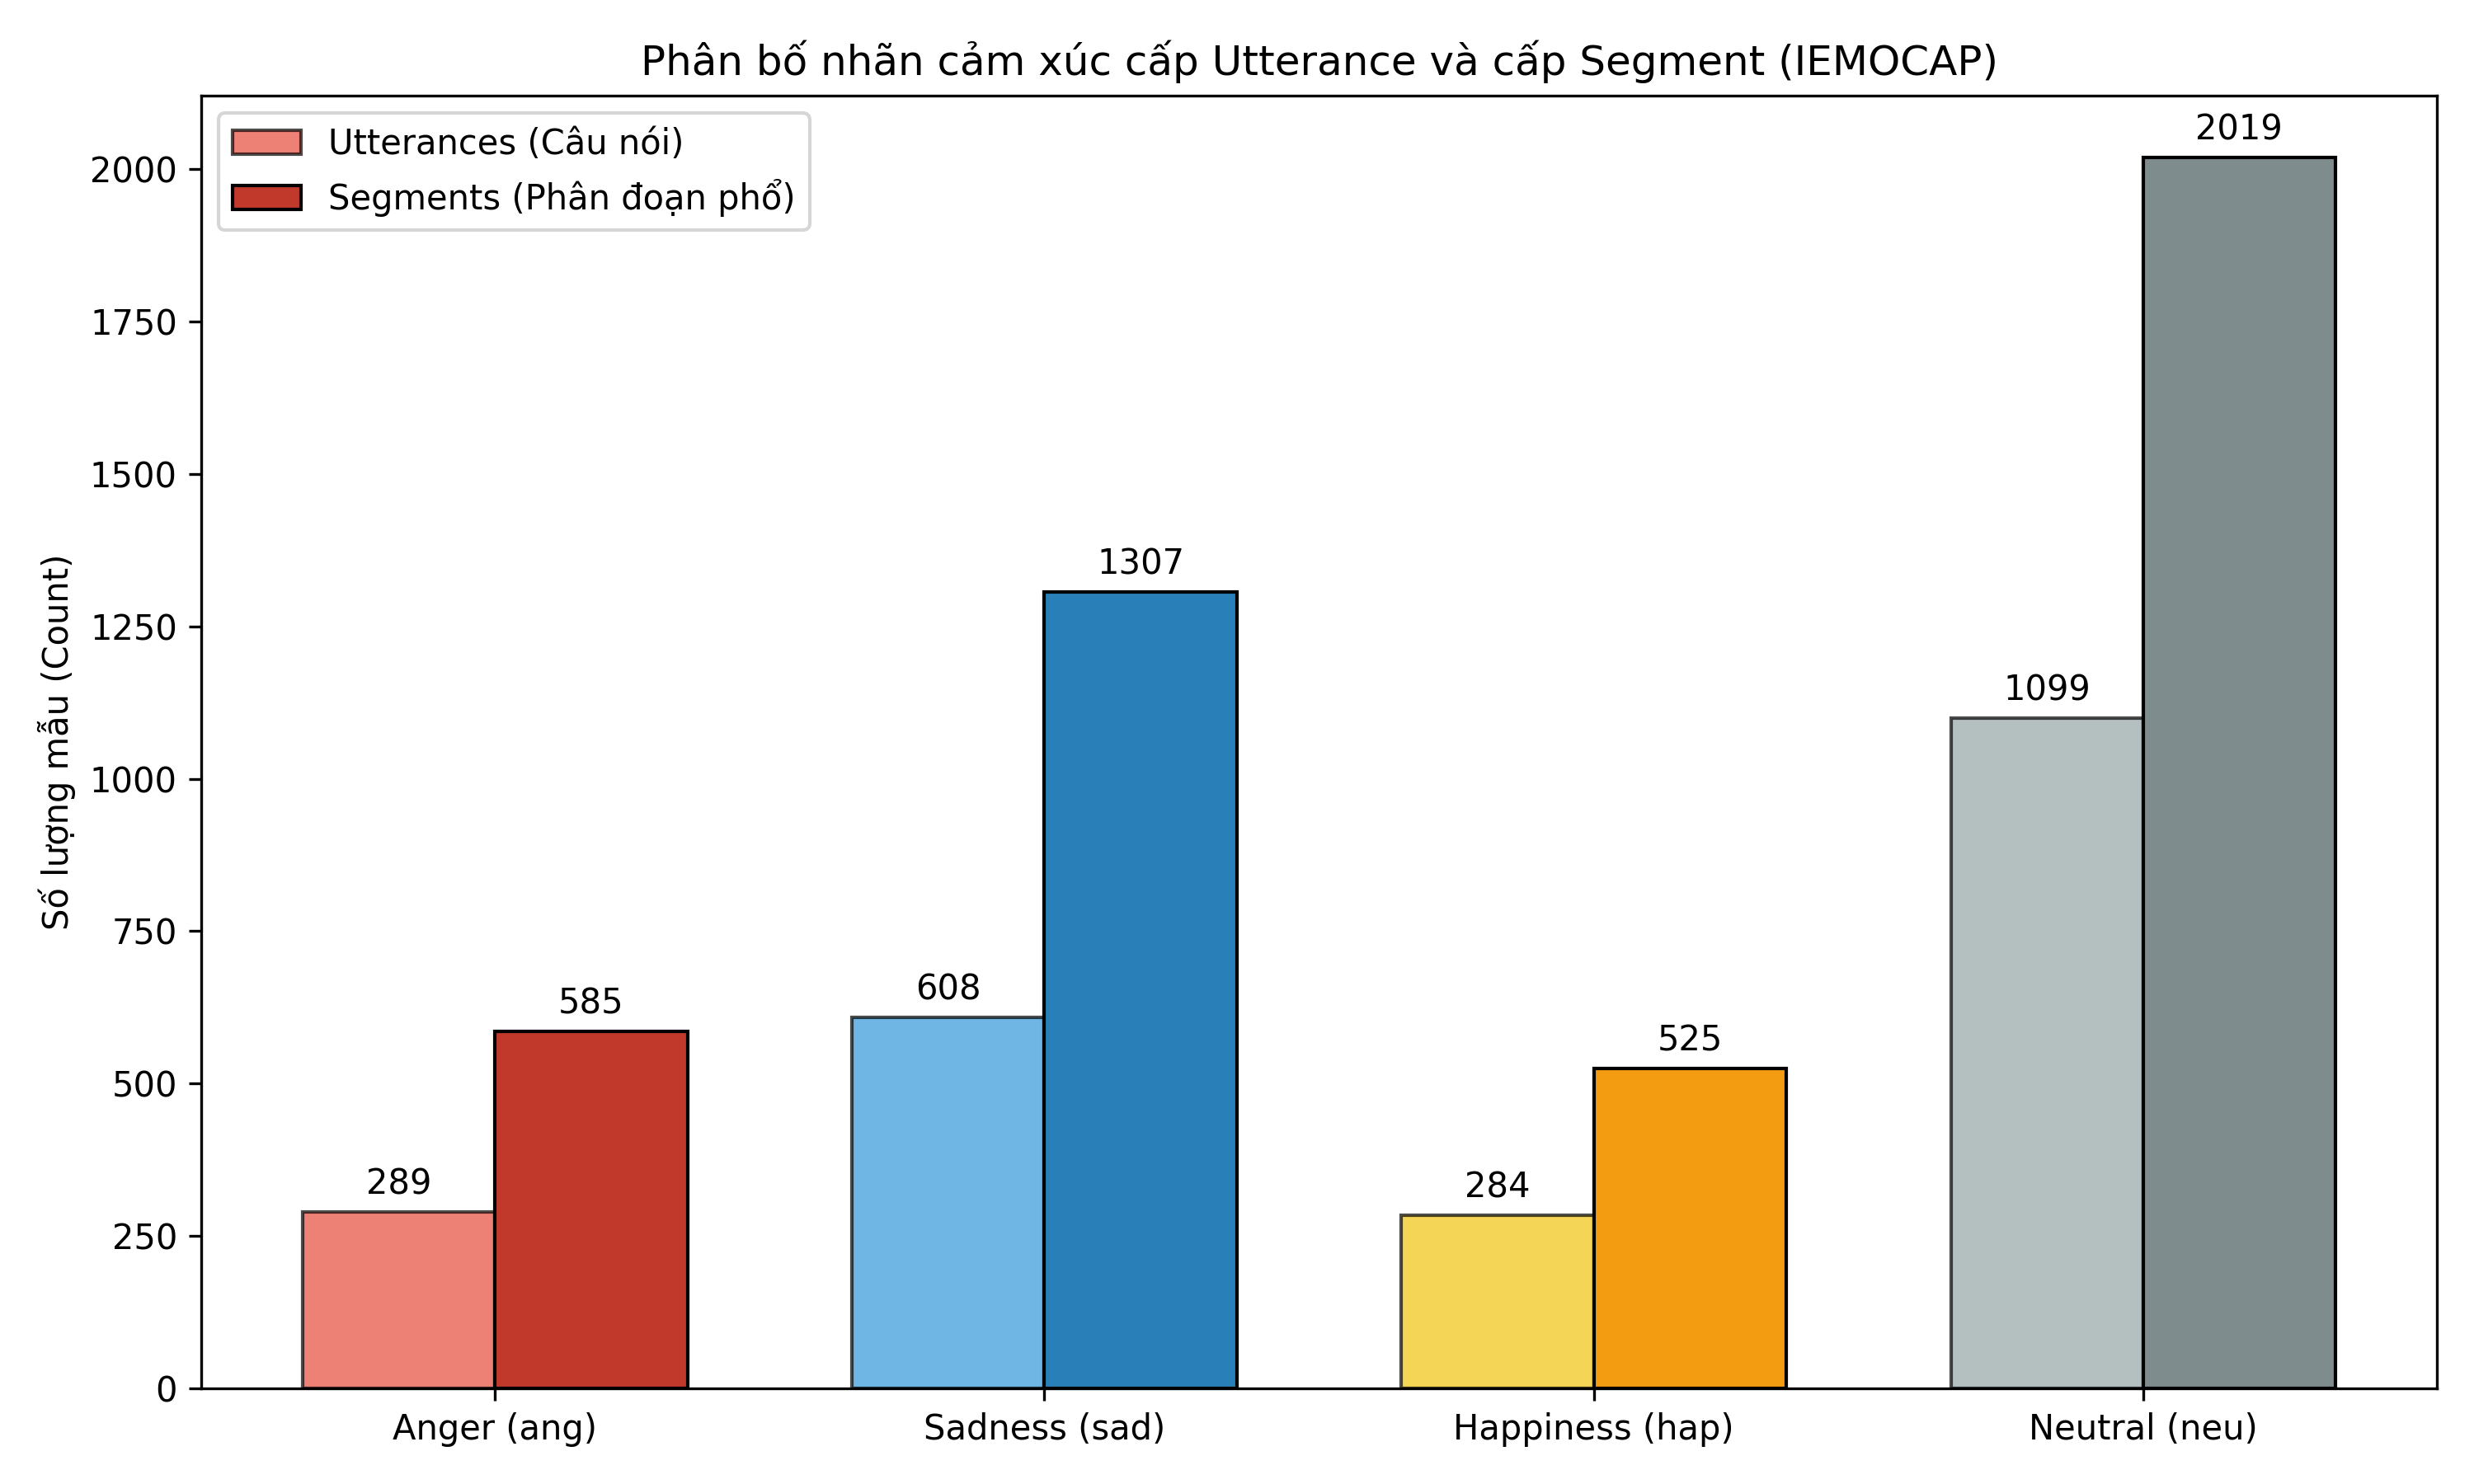
\includegraphics[width=0.75\textwidth]{data_distribution.png}
    \caption{Biểu đồ phân bổ mẫu theo nhãn cảm xúc và theo speaker}
    \label{fig:data_distribution}
\end{figure}

\begin{figure}[H]
    \centering
    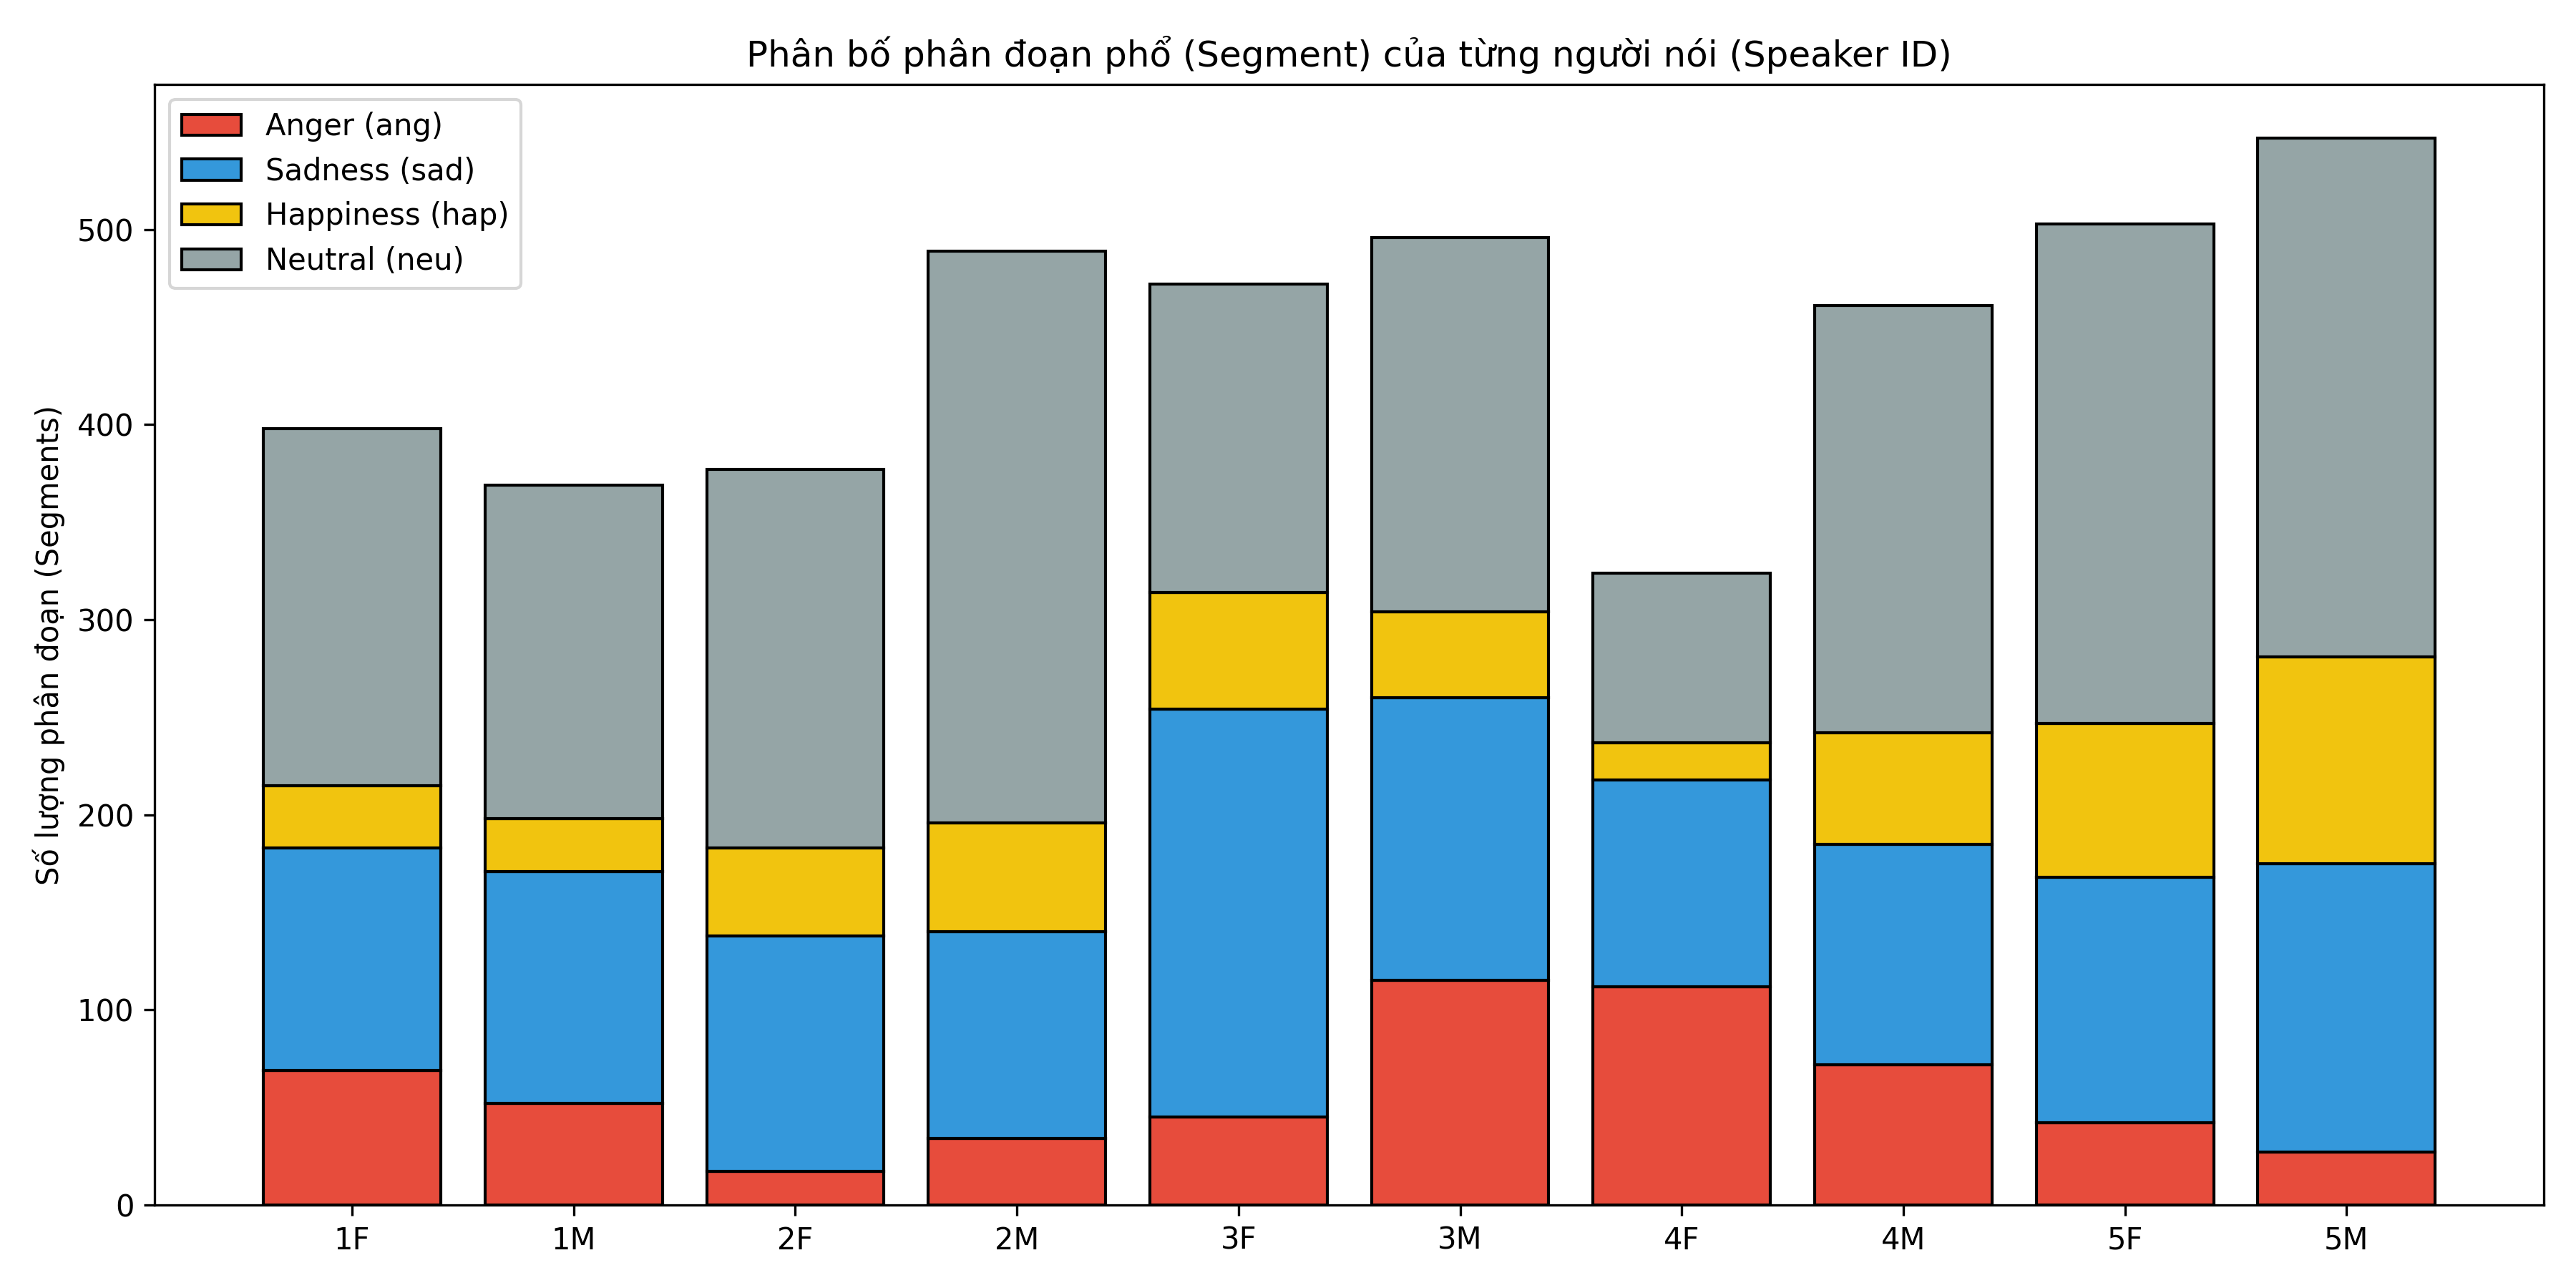
\includegraphics[width=0.75\textwidth]{speaker_distribution.png}
    \caption{Phân bổ mẫu theo từng speaker trong 5 Session}
    \label{fig:speaker_distribution}
\end{figure}

Sự chênh lệch lớn giữa lớp đa số (Neutral: 48,2\%) và lớp thiểu số nhất (Happiness: 12,5\%) lên đến gần 4 lần, đặt ra thách thức lớn về sự mất cân bằng dữ liệu đối với mô hình phân loại. Phân bổ mẫu cụ thể theo từng diễn viên và theo từng session được trực quan hóa lần lượt trong Hình~\ref{fig:data_distribution} và Hình~\ref{fig:speaker_distribution}.


\section{Quy trình tiền xử lý dữ liệu}
\label{sec:preprocessing}

\subsection{Bước 1: Trích xuất đặc trưng Log-Spectrogram}

Quy trình trích xuất đặc trưng được thực hiện thông qua module \path{features_extraction/} sử dụng thư viện \texttt{librosa} \cite{mcfee2015} theo các bước tuần tự bao gồm: resampling tín hiệu về tần số lấy mẫu chuẩn 16 kHz; áp dụng bộ lọc tiền nhấn với hệ số $\alpha = 0.97$; thực hiện phép biến đổi STFT sử dụng cửa sổ Hamming độ dài 40 ms và bước trượt 10 ms với $N_{\text{FFT}} = 800$; thực hiện chuyển đổi biên độ sang thang đo decibel; và cuối cùng là giữ lại 200 băng tần số thấp nhất để tạo thành ma trận đặc trưng Log-Spectrogram.

\subsection{Bước 2: Phân đoạn (Segmentation)}

Do mỗi câu nói có thời lượng khác nhau, ma trận phổ đồ tương ứng sẽ có chiều dài thời gian khác nhau. Để đưa dữ liệu vào huấn luyện mạng CNN một cách hiệu quả, hệ thống tiến hành cắt ma trận phổ đồ thành các phân đoạn độc lập có kích thước cố định $200 \times 300$, tương đương khoảng 3 giây âm thanh. Đối với các câu nói ngắn hơn 300 khung thời gian, việc đệm để đạt chiều dài chuẩn sẽ được thực hiện sau bước chuẩn hóa MinMax về dải $[0.0, 1.0]$ bằng cách đệm thêm giá trị $0.0$ (tương ứng với mức năng lượng tối thiểu $-80\,\text{dB}$ ban đầu). Phương pháp này giúp tránh hiện tượng đệm trực tiếp giá trị $0$ trên thang decibel vốn biểu thị mức năng lượng âm học cực đại ($0\,\text{dB}$). Phân bổ mẫu ở cấp phân đoạn được tổng hợp chi tiết trong Bảng~\ref{tab:segment_distribution}.

\begin{table}[H]
\centering
\caption{Thống kê phân bổ mẫu theo nhãn cảm xúc (cấp phân đoạn)}
\label{tab:segment_distribution}
\begin{tabular}{lcc}
\toprule
\textbf{Nhãn cảm xúc} & \textbf{Số phân đoạn} & \textbf{Tỉ lệ (\%)} \\
\midrule
Neutral & 2.019 & 45,5 \\
Sadness & 1.307 & 29,5 \\
Anger & 585 & 13,2 \\
Happiness & 525 & 11,8 \\
\midrule
\textbf{Tổng cộng} & \textbf{4.436} & \textbf{100,0} \\
\bottomrule
\end{tabular}
\end{table}

\subsection{Bước 3: Chuẩn hóa và định dạng ảnh đầu vào}

Quy trình chuẩn hóa và định dạng ảnh đầu vào được thiết lập qua ba bước chính. Trước tiên, hệ thống áp dụng chuẩn hóa MinMax trên tập Train để chuyển đổi dải giá trị decibel của phổ đồ từ $[-80\,\text{dB}, 0\,\text{dB}]$ về khoảng $[0.0, 1.0]$, cùng bộ scaler này sau đó được áp dụng đồng bộ cho tập Validation và tập Test. Sau đó, phần đệm thời gian cho các câu ngắn sẽ được điền giá trị $0.0$ để đưa về kích thước chuẩn $200 \times 300$. Tiếp theo, đặc trưng được chuyển đổi sang dạng Pseudo-RGB bằng cách lật ngược trục tần số và nhân bản kênh đơn thành 3 kênh giống nhau để tạo thành tensor kích thước $(3 \times 200 \times 300)$. Cuối cùng, tensor được resize về kích thước chuẩn $256 \times 256$ pixels và thực hiện chuẩn hóa Z-Score theo các giá trị trung bình và độ lệch chuẩn của bộ dữ liệu ImageNet. 

Cần lưu ý rằng việc nhân bản kênh đơn thành 3 kênh để áp dụng mô hình pre-trained từ ImageNet tồn tại một hạn chế về mặt lý thuyết (domain mismatch). ImageNet chứa các hình ảnh tự nhiên có tính chất bất biến tịnh tiến không gian (spatial translation invariance), trong khi phổ đồ âm thanh là biểu diễn thời gian-tần số (time-frequency) mà việc dịch chuyển theo trục dọc làm thay đổi cao độ (pitch) và thay đổi ngữ nghĩa. Thêm vào đó, việc nhân bản 3 kênh giống hệt nhau khiến các bộ lọc tích chập ở lớp đầu tiên nhận thông tin thừa. Tuy nhiên, phương pháp này được chấp nhận rộng rãi như một kỹ thuật kỹ nghệ thực hành thông dụng, giúp tận dụng các bộ lọc thô đã được tối ưu trước (như phát hiện các đường biên, vân bề mặt và kết cấu) từ ImageNet để học các họa âm (harmonics) và điểm chuyển tiếp trên phổ đồ nhanh hơn.


\section{Phân chia dữ liệu Speaker-Independent}
\label{sec:speaker_independent}

Để đảm bảo mô hình có khả năng tổng quát hóa tốt trên giọng nói của người lạ (người nói không xuất hiện trong tập huấn luyện), dữ liệu được phân chia theo nguyên tắc Speaker-Independent nghiêm ngặt như được mô tả trong Bảng~\ref{tab:speaker_split}.

\begin{table}[H]
\centering
\caption{Phân chia dữ liệu theo Speaker-Independent}
\label{tab:speaker_split}
\begin{tabular}{lll}
\toprule
\textbf{Tập dữ liệu} & \textbf{Số speaker} & \textbf{Mô tả} \\
\midrule
Train & 8 speakers (4 sessions) & Huấn luyện mô hình \\
Validation & 1 speaker & Chọn mô hình tốt nhất \\
Test & 1 speaker & Đánh giá cuối cùng \\
\bottomrule
\end{tabular}
\end{table}

Ví dụ, với cấu hình mặc định (val=1F, test=1M), 8 speakers từ Session 2--5 được sử dụng làm tập huấn luyện, diễn viên nữ của Session 1 (1F) làm validation, và diễn viên nam của Session 1 (1M) làm tập test. Để ngăn chặn hoàn tượng rò rỉ dữ liệu (data leakage) giữa các tập dữ liệu, quy trình phân chia theo danh tính người nói (Speaker ID) được thực hiện một cách nghiêm ngặt trên cấp độ câu nói (Utterance) trước khi cắt phân đoạn.

Tuy nhiên, thiết lập phân chia này vẫn tồn tại một hạn chế âm học thực tế. Do diễn viên validation (nữ) và diễn viên test (nam) trong mỗi cấu hình thuộc về cùng một Session (ví dụ Session 1), hai người này nói chuyện trực tiếp trong cùng một phòng thu với cùng hệ thống microphone và nhiễu nền tĩnh. Do đó, mô hình có thể vô tình khai thác các đặc tính tĩnh của kênh truyền (channel characteristics) hoặc nhiễu phòng chung từ tập validation để cải thiện dự đoán trên tập test. Đây là một dạng rò rỉ âm học môi trường nhẹ (acoustic environment leakage) làm giảm phần nào tính độc lập môi trường tuyệt đối của hệ thống kiểm thử, và sẽ được khắc phục bằng phương pháp Leave-One-Session-Out (LOSO) thực thụ trong các nghiên cứu tiếp theo. Danh sách cụ thể của 10 diễn viên trong bộ dữ liệu được liệt kê trong Bảng~\ref{tab:speakers}.

\begin{table}[H]
\centering
\caption{Danh sách 10 Speaker trong IEMOCAP}
\label{tab:speakers}
\begin{tabular}{cccc}
\toprule
\textbf{Session} & \textbf{Speaker ID} & \textbf{Giới tính} & \textbf{Ký hiệu} \\
\midrule
Session 1 & Speaker 1 & Nữ / Nam & 1F / 1M \\
Session 2 & Speaker 2 & Nữ / Nam & 2F / 2M \\
Session 3 & Speaker 3 & Nữ / Nam & 3F / 3M \\
Session 4 & Speaker 4 & Nữ / Nam & 4F / 4M \\
Session 5 & Speaker 5 & Nữ / Nam & 5F / 5M \\
\bottomrule
\end{tabular}
\end{table}


\section{Kiến trúc mô hình}
\label{sec:model_architecture}

Tất cả các mô hình CNN được xây dựng trong đồ án đều kế thừa một giao diện đồng nhất để dễ dàng tích hợp và đánh giá. Cụ thể, các mô hình nhận đầu vào là tensor kích thước $(N, 3, 256, 256)$ đại diện cho batch ảnh phổ đồ Pseudo-RGB đã chuẩn hóa và trả về đầu ra là các logits kích thước $(N, 4)$ tương ứng với 4 lớp cảm xúc. Các mô hình được khởi tạo sử dụng trọng số pre-trained từ ImageNet để chuyển giao tri thức và chỉ thực hiện sửa đổi lớp phân loại kết nối đầy đủ cuối cùng phù hợp với số lượng lớp cảm xúc của bài toán. Chi tiết tổng hợp về số lượng tham số và đặc điểm của các mô hình được trình bày trong Bảng~\ref{tab:model_summary}.

\begin{table}[H]
\centering
\caption{Tổng hợp các kiến trúc mô hình}
\label{tab:model_summary}
\begin{tabular}{lllr}
\toprule
\textbf{Mô hình} & \textbf{Đặc điểm chính} & \textbf{Lớp phân loại} & \textbf{Tham số} \\
\midrule
AlexNet & 5 Conv + 3 FC & FC(4096, 4) & 57,02M \\
AlexNet GAP & 5 Conv + GAP & Conv $1\times1$ + AvgPool & 2,47M \\
ResNet-18 & Skip Connection & FC(512, 4) & 11,18M \\
DenseNet-121 & Dense Block & FC(1024, 4) & 6,96M \\
EfficientNet-B0 & Compound Scaling & FC(1280, 4) & 4,01M \\
MobileNet-V2 & Depthwise Conv & FC(1280, 4) & 2,23M \\
\bottomrule
\end{tabular}
\end{table}


\section{Quy trình huấn luyện}
\label{sec:training_procedure}

\subsection{Cấu hình huấn luyện}

Bảng~\ref{tab:training_config} trình bày cấu hình siêu tham số huấn luyện được thiết lập đồng nhất cho tất cả các mô hình trong các lượt thực nghiệm nhằm đảm bảo tính công bằng của các so sánh.

\begin{table}[H]
\centering
\caption{Cấu hình huấn luyện chung}
\label{tab:training_config}
\begin{tabular}{ll}
\toprule
\textbf{Tham số} & \textbf{Giá trị} \\
\midrule
Optimizer & AdamW \\
Learning rate & $10^{-4}$ \\
Batch size & 64 \\
Epochs & 60 \\
Random seed & 100 \\
GPU & NVIDIA RTX 3060 (12GB) \\
Framework & PyTorch \\
\bottomrule
\end{tabular}
\end{table}

\subsection{Chiến lược chọn mô hình tốt nhất}

Sau mỗi epoch huấn luyện, mô hình được đánh giá trực tiếp trên tập Validation. Để giải quyết triệt để vấn đề mất cân bằng dữ liệu, hệ thống tự động theo dõi và lưu lại cấu hình trọng số tương ứng với kết quả Unweighted Accuracy (UA) đạt giá trị cao nhất trên tập Validation thay vì dựa vào chỉ số Weighted Accuracy nhằm tránh việc mô hình bị thiên lệch vào lớp đa số. Khi kết thúc quá trình huấn luyện, cấu hình trọng số tối ưu này sẽ được nạp lại để tiến hành đánh giá khách quan trên tập kiểm thử độc lập.

\subsection{Chiến lược đánh giá cấp câu nói (Utterance-level)}

Do mỗi câu nói có thể được phân cắt thành nhiều phân đoạn khác nhau, việc dự đoán nhãn cảm xúc ở cấp câu nói được thực hiện bằng cách tính trung bình hóa xác suất dự đoán (log-softmax) của toàn bộ các phân đoạn thuộc cùng một câu nói, sau đó áp dụng phép lấy cực đại (argmax):
\begin{equation}
    \hat{y}_u = \argmax_c \left( \frac{1}{|\mathcal{S}_u|} \sum_{s \in \mathcal{S}_u} \log P(c | s) \right)
    \label{eq:utt_pred}
\end{equation}
trong đó $\mathcal{S}_u$ là tập hợp tất cả các phân đoạn được cắt ra từ câu nói $u$.


\section{Các chỉ số đánh giá}
\label{sec:metrics}

Hiệu năng của mô hình được đánh giá toàn diện qua ba chỉ số chính. Đầu tiên là Weighted Accuracy (WA) đo lường tỉ lệ dự đoán chính xác trên tổng số mẫu thực tế. Chỉ số thứ hai là Unweighted Accuracy (UA) được tính bằng trung bình cộng độ chính xác của từng lớp cảm xúc độc lập không phụ thuộc vào số lượng mẫu của mỗi lớp, phản ánh chính xác khả năng phân loại đồng đều trên dữ liệu mất cân bằng. Cuối cùng, ma trận nhầm lẫn (Confusion Matrix) kích thước $4 \times 4$ được sử dụng để trực quan hóa số lượng mẫu phân loại đúng và sai lệch giữa các cặp lớp cảm xúc, giúp xác định chi tiết điểm yếu của từng mô hình.
